\documentclass[t,aspectratio=32]{beamer}

\usepackage{listings}
\usepackage{graphicx}
\usepackage{tikz}
\usepackage{xcolor}

\definecolor{bp-blue} {RGB}{  2, 103, 193}
\definecolor{bp-green}{RGB}{ 35, 150, 127}
\definecolor{bp-grey} {RGB}{145, 129, 117}
\definecolor{bp-red}  {RGB}{254,  95,  85}

\lstdefinestyle{bpstyle}{
    literate={*}{*}1
}
\lstset{
    basicstyle=\footnotesize,
    breaklines=true,
    captionpos=b,
    commentstyle=\color{bp-grey},
    mathescape=true,
    showstringspaces=false,
    stringstyle=\color{bp-green},
    style=bpstyle
}
\lstloadlanguages{java,xml}

\lstdefinestyle{antlr}{
    breaklines=true,
    moredelim=[s][\color{bp-green}\ttfamily]{'}{'},
    commentstyle={\color{bp-grey}\itshape},
    morecomment=[l]{//},
    morekeywords={grammar}
    keywordstyle={\color{bp-blue}},
}

\newcommand{\p}[1]{{\left(#1\right)}}

\usetheme{default}
\beamertemplatenavigationsymbolsempty\setbeamersize{
    text margin left=0.5cm,
    text margin right=0.5cm
}
\addtobeamertemplate{frametitle}{\vspace*{0.2em}\hspace*{0.2em}}{\vspace*{0.5em}}

\setbeamerfont{title}{size=\LARGE,
                      series=\bfseries,
                      family=\rmfamily}
\setbeamerfont{frametitle}{size=\Large}

\setbeamercolor{title}{fg=black}
\setbeamercolor{frametitle}{fg=black}
\setbeamercolor{itemize item}{fg=black}
\setbeamercolor{itemize subitem}{fg=black}
\setbeamercolor{itemize subsubitem}{fg=black}
\setbeamercolor{enumerate item}{fg=black}
\setbeamercolor{enumerate subitem}{fg=black}
\setbeamercolor{enumerate subsubitem}{fg=black}
\setbeamercolor{block body example}{fg=black!90,
                                    bg=black!10}
\setbeamercolor{block title example}{fg=white,
                                     bg=black!30}

\setbeamertemplate{itemize item}[circle]
\setbeamertemplate{blocks}[shadow=true]

\title{Bachelor Project SP 2021}
\subtitle{Expression Generator}
\author{Bevilacqua Joey}
\institute{Universit\`a della Svizzera Italiana}
\date{June 18, 2021}

\begin{document}

% ------------------------------

% 1.0
\begin{frame}
\maketitle
\end{frame}

% ------------------------------

% 2.0
\begin{frame}
\frametitle{Expressions}

\begin{itemize}
\item Combine values with functions and operators to produce other values
\item Programming languages define rules that determine how expressions are
      combined and evaluated to perform tasks
\end{itemize}
\end{frame}

% 2.1
\begin{frame}
\frametitle{Expressions}

\begin{itemize}
\item Combine values with functions and operators to produce other values
\item Programming languages define rules that determine how expressions are
      combined and evaluated to perform tasks
\item Expression Tutor aids students understanding expressions by providing
      worked examples and exercises
\item Writing all of that is time–consuming and error–prone, we should
      get a computer to do it
\end{itemize}
\end{frame}


% ------------------------------

% 3.0
\begin{frame}
\frametitle{Generating expressions}

``\textit{Computer, please generate an expression for me}''
\end{frame}

% 3.1
\begin{frame}
\frametitle{Generating expressions}

``\textit{Computer, please generate an expression for me}''
\vspace{1em}
\begin{enumerate}
\item What language do you want me to speak? (Grammars)
\item What do you want me to say? (Constraints)
\item How do you want me to say it? (Interfaces)
\end{enumerate}
\end{frame}

% ------------------------------

% 4.0
\begin{frame}
\frametitle{1. What language do you want me to speak? – Grammars}

\begin{itemize}
\item Language agnosticism
\item Context–Free–Grammars: $ R \to s $
    \begin{itemize}
    \item $ R $: terminal (``name'' of the rule)
    \item $ s $: set of symbols that identify other rules or terminals
    \end{itemize}
\item Grammars can be used to describe any valid string for the language
      it defines
\end{itemize}
\end{frame}

% 4.1
\begin{frame}[fragile]
\frametitle{1. What language do you want me to speak? – Grammars}

\textbf{Context–Free–Grammars}

\begin{lstlisting}[style=antlr]
E $ \to $ E '+' E
E $ \to $ E '-' E
E $ \to $ E '*' E
E $ \to $ E '/' E
E $ \to $ 0
E $ \to $ 1
$ \hdots $
\end{lstlisting}
\end{frame}

% 4.2
\begin{frame}[fragile]
\frametitle{1. What language do you want me to speak? – Grammars}

\textbf{ANTLR grammars}

\begin{lstlisting}[style=antlr]
expr: SUBJECT 'like' (targets | target);
targets: targets ', ' target
       | target 'and' target;
target: 'the color ' COLOR
      | 'the number ' NUM;
SUBJECT: 'I' | 'you' | 'we';
COLOR: 'red' | 'green' | 'blue';
NUM: '0' | [1-9] [0-9]*;
\end{lstlisting}
\end{frame}

% 4.3
\begin{frame}
\frametitle{1. What language do you want me to speak? – Grammars}

Parsing: ``\textit{I like the color red and the number 2}''
\begin{center}
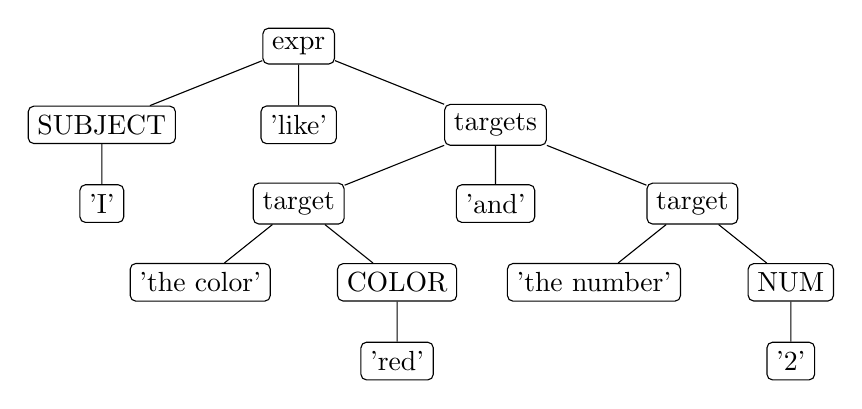
\begin{tikzpicture}[level distance=1cm, sibling distance=2.5cm]
\tikzstyle{every node}+=[draw, rectangle, rounded corners=2pt]
\node (a)[node distance=4cm] {expr}
    child { node { SUBJECT }
        child { node { 'I' } }
    }
    child { node { 'like' } }
    child { node { targets }
        child { node { target }
            child { node { 'the color' } }
            child { node { COLOR }
                child { node { 'red' } }
            }
        }
        child { node { 'and' } }
        child { node { target }
            child { node { 'the number' } }
            child { node { NUM } 
                child { node { '2' } }
            }
        }
    }
    ;
\end{tikzpicture}
\end{center}
\end{frame}

% 4.4
\begin{frame}
\frametitle{1. What language do you want me to speak? – Grammars}

\textbf{Abstract and Concrete syntax trees}
\begin{center}
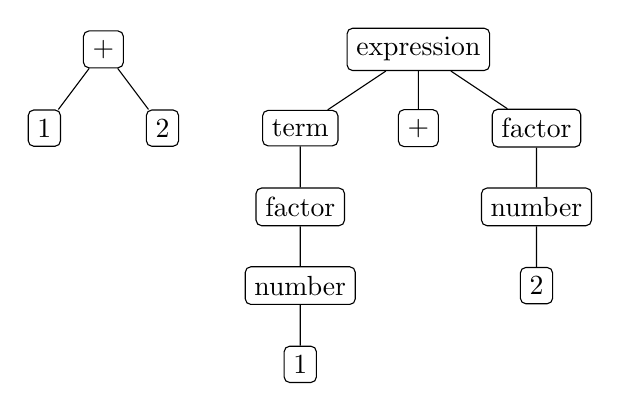
\begin{tikzpicture}[
    level 1/.style={level distance=1cm},
    level 2/.style={level distance=1cm},
    level 3/.style={level distance=1cm}]
\tikzstyle{every node}+=[draw, rectangle, rounded corners=2pt]
\node (a) {+}
      child { node { 1 } }
      child { node { 2 } }
      ;
\node (b)[right of=a, node distance=4cm] {expression}
      child { node { term }
            child { node { factor }
                  child { node { number } 
                        child { node { $ 1 $ } }
                  }
            }
      }
      child { node { + } }
      child { node { factor }
            child { node { number } 
                  child { node { $ 2 $ } }
            }
      }
      ;
\end{tikzpicture}
\end{center}
\end{frame}

% ------------------------------

% 5.0
\begin{frame}
\frametitle{2. What do you want me to say? – Constraints}

\begin{enumerate}
\item Starting rule: defines the overall ``structure'' of the generated
      expression
\item Include rule: include a specific rule in the generated expression
\item Tree size: control the Concrete Syntax Tree depth and ``width''
\end{enumerate}
\end{frame}

% 5.1
\begin{frame}
\frametitle{2. What do you want me to say? – Constraints}

\begin{enumerate}
\item Starting rule: defines the overall ``structure'' of the generated
      expression
\item Include rule: include a specific rule in the generated expression
\item Tree size: control the Concrete Syntax Tree depth and ``width''
    \begin{itemize}
    \item Can be thought of as a ``complexity'' factor
    \item Depth: challenging because of language agnosticism (some languages
          have implicit depth constraints that the user may be unaware of)
    \item Width: control how many rule repetitions (``star'' and ``plus'') are
          allowed during the expression generation
    \end{itemize}
\end{enumerate}
\end{frame}

% 5.2
\begin{frame}
\frametitle{2. What do you want me to say? – Constraints}

\begin{center}
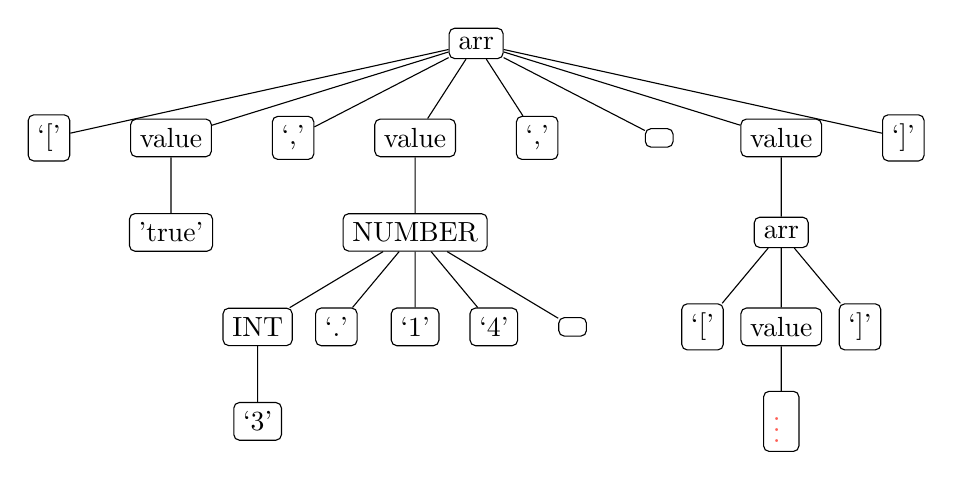
\begin{tikzpicture}[level distance=1.2cm, sibling distance=1.55cm,
                    level 3/.style={sibling distance=1cm}]
\tikzstyle{every node}+=[draw, rectangle, rounded corners=2pt]
\node (a) {arr}
      child { node { `[' } }
      child { node { value } 
              child { node { 'true' } } }
      child { node { `,' } }
      child { node { value }
              child { node { NUMBER } 
                    child { node { INT }
                            child { node { `3' } }
                    }
                    child { node { `.' } }
                    child { node { `1' } }
                    child { node { `4' } }
                    child { node { {\color{bp-red} $ \hdots $ } } }
              }
      }
      child { node { `,' } }
      child { node { {\color{bp-red} $ \hdots $ } } }
      child { node { value }
              child { node { arr } 
                      child { node { `[' } }
                      child { node { value }
                              child { node { {\color{bp-red} $ \vdots $ } } }
                      }
                      child { node { `]' } }
              }
      }
      child { node { `]' } }
      ;
\end{tikzpicture}
\end{center}
\end{frame}

% ------------------------------

% 6.0
\begin{frame}
\frametitle{3. How do you want me to say it? – Interfaces}

\begin{itemize}
\item Command line interface
\item Web interface
    \begin{itemize}
    \item Web API
    \item Expression Tutor
    \end{itemize}
\end{itemize}
\end{frame}

% 6.1
\begin{frame}
\frametitle{3. How do you want me to say it? – Interfaces}

\textbf{Command line interface}

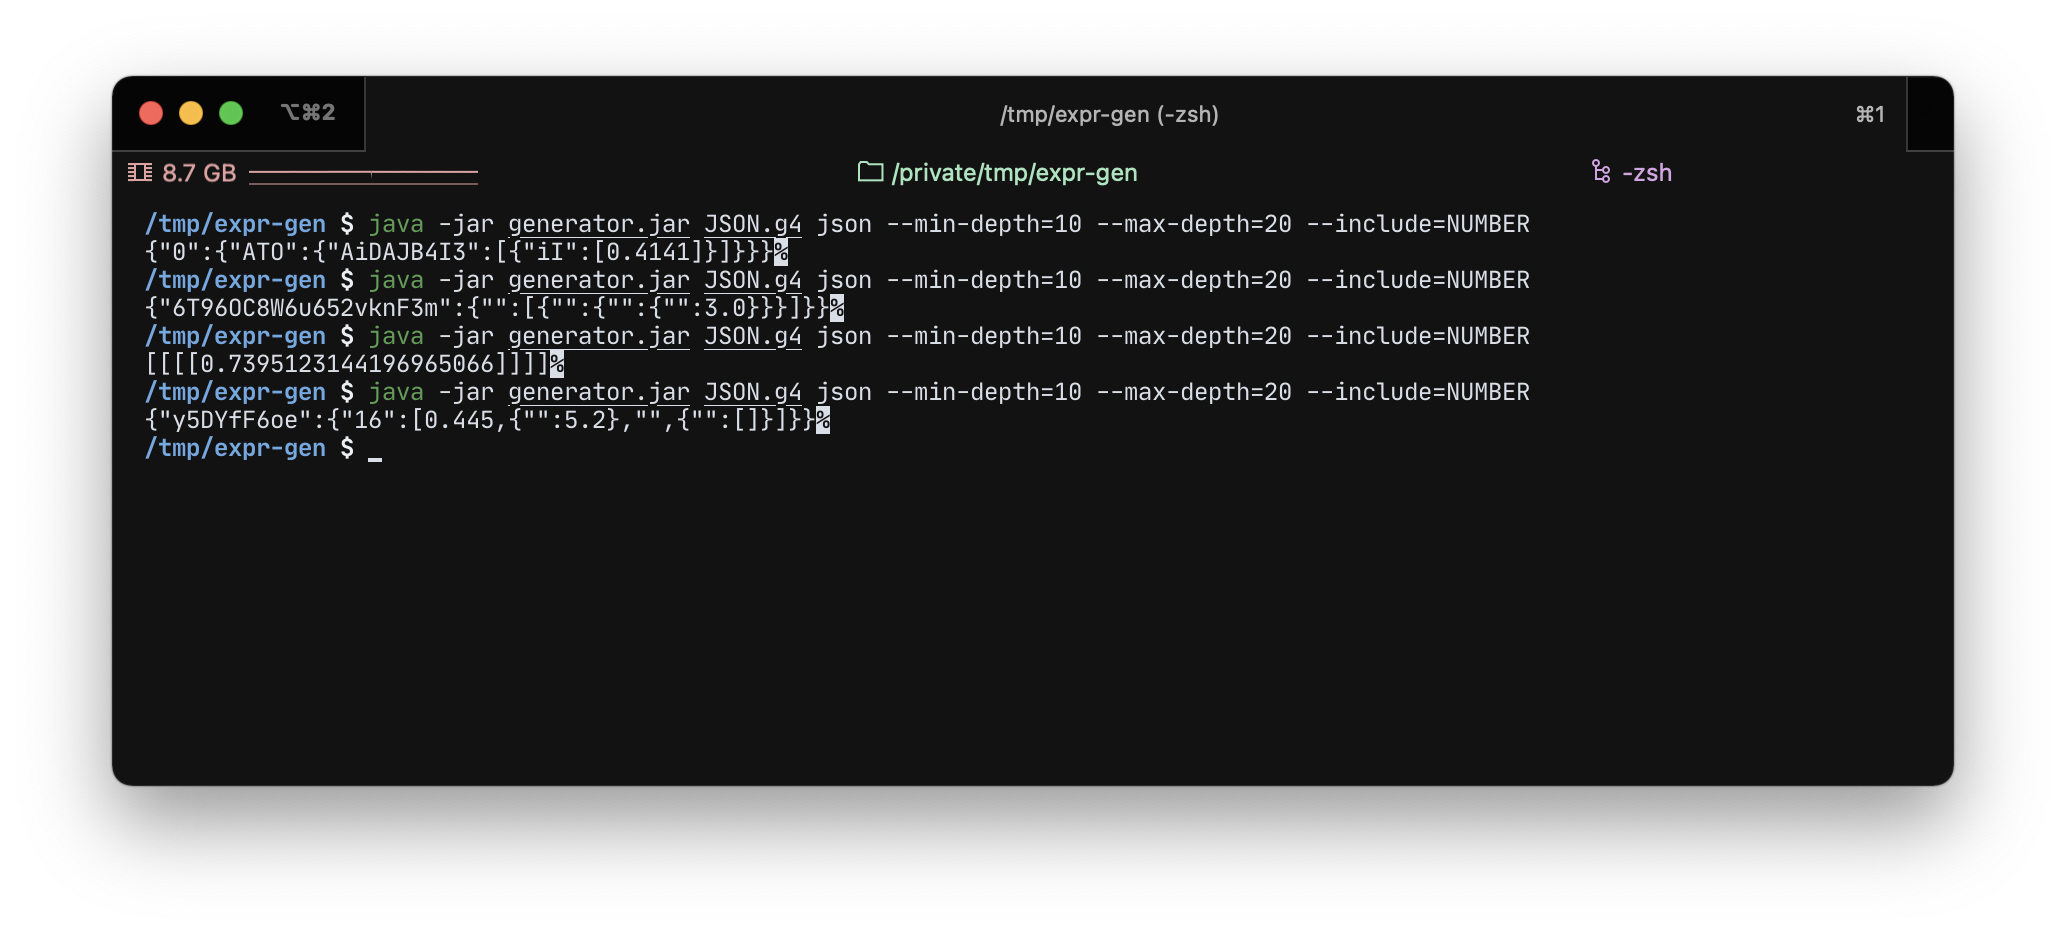
\includegraphics[width=\textwidth]{img/cli_show.png}
\end{frame}

% 6.2
\begin{frame}
\frametitle{3. How do you want me to say it? – Interfaces}

\textbf{Command line interface}: debug mode

\begin{center}
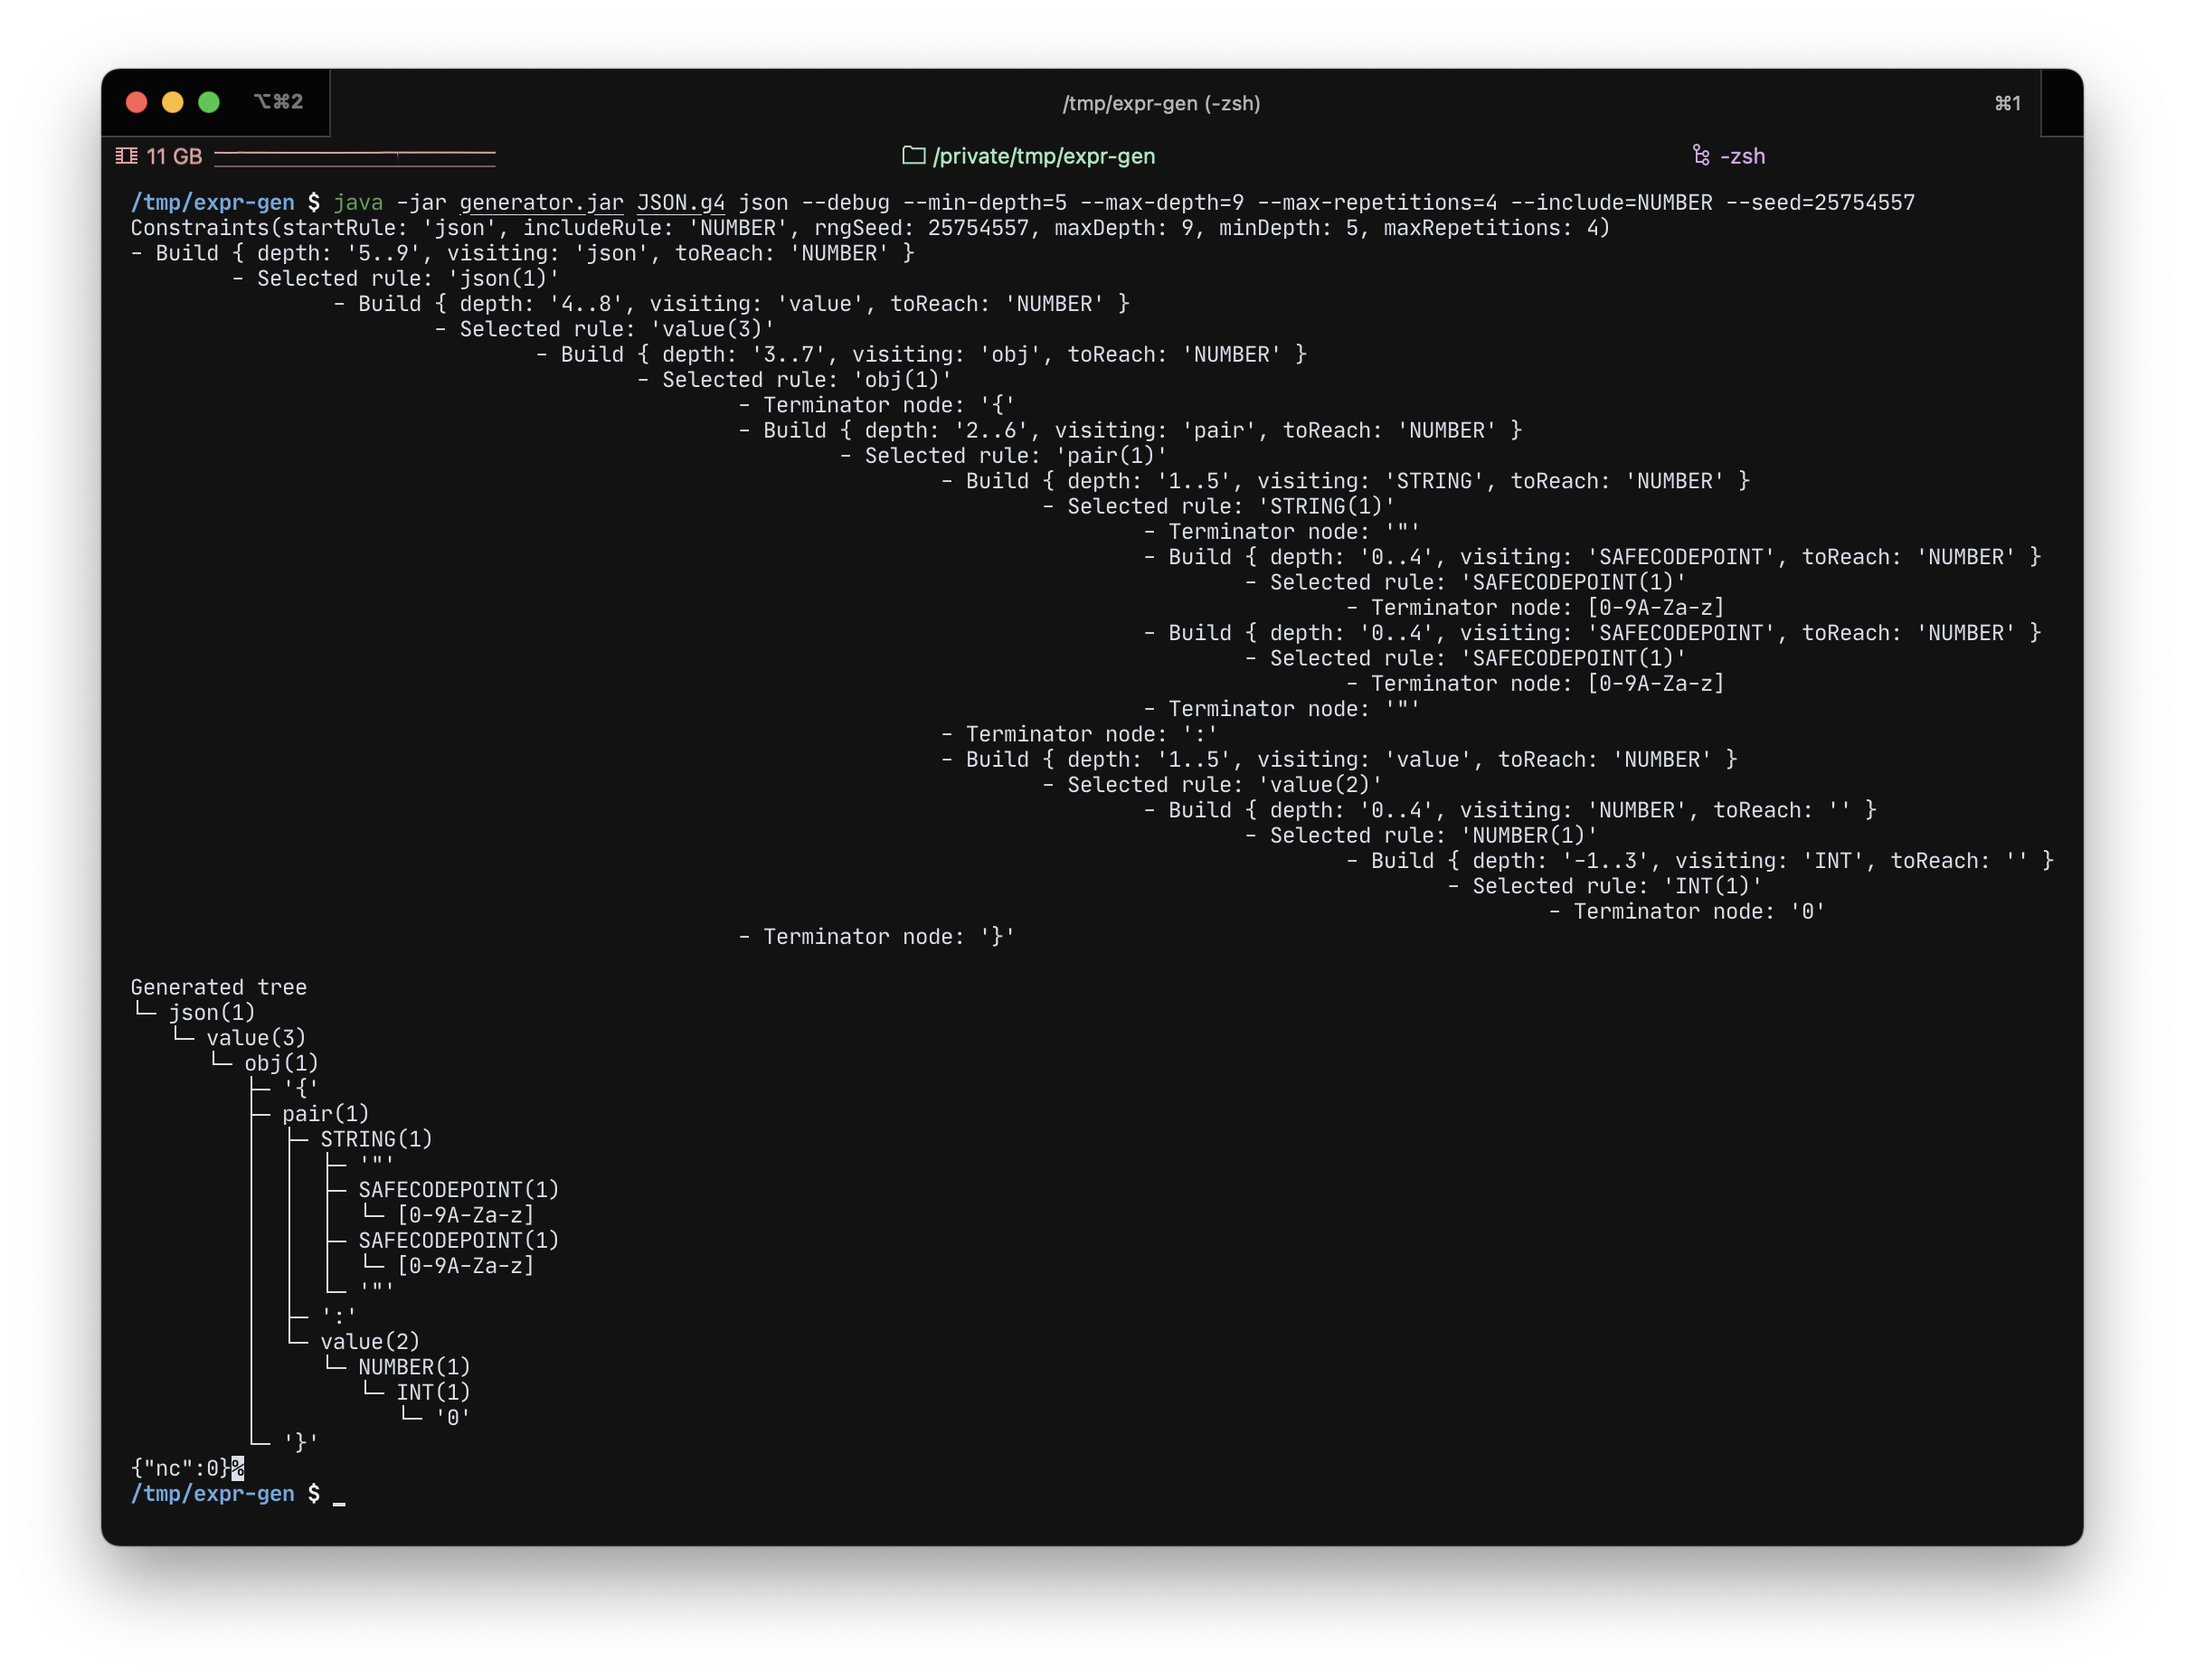
\includegraphics[height=18em]{img/cli_debug.png}
\end{center}
\end{frame}

% 6.3
\begin{frame}
\frametitle{3. How do you want me to say it? – Interfaces}

\textbf{Command line interface}: integrate in workflows with
unix pipes

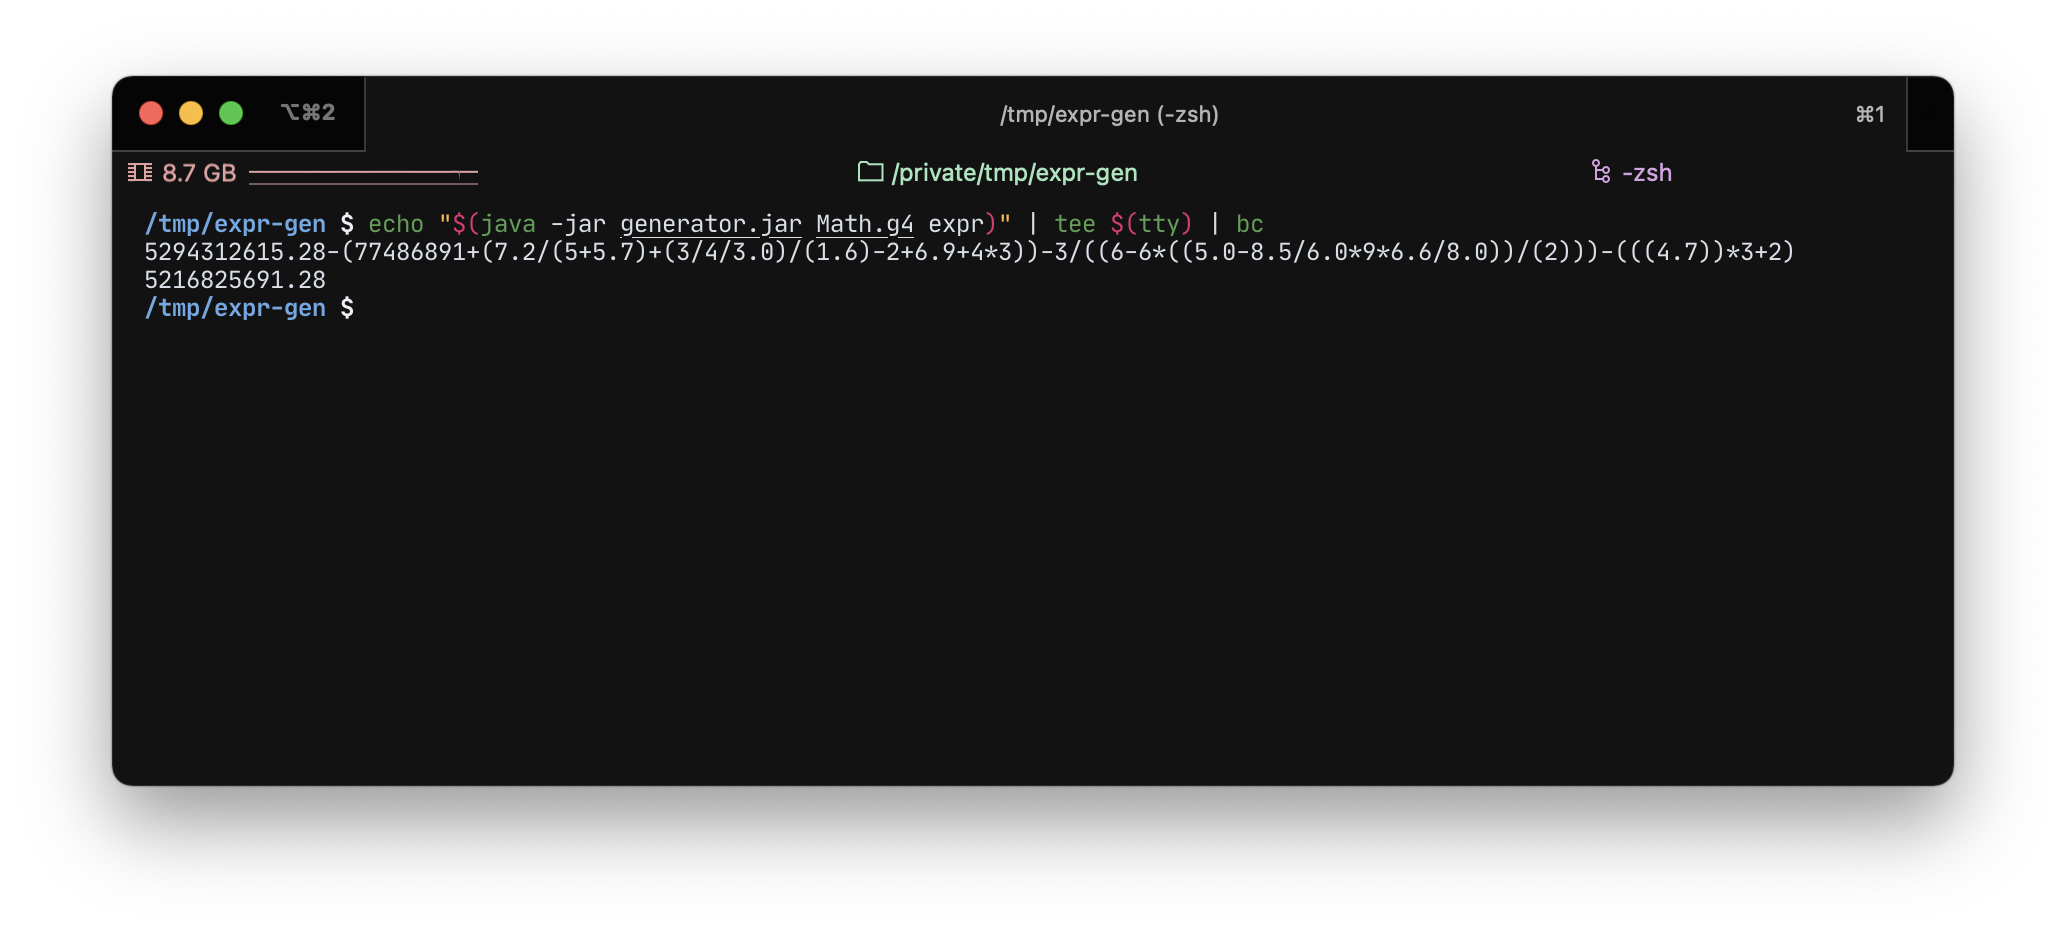
\includegraphics[width=\textwidth]{img/cli_pipes.png}
\end{frame}

% 6.4
\begin{frame}
\frametitle{3. How do you want me to say it? – Interfaces}

\textbf{Web interface}: Expression Tutor uses the web APIs to
generate expressions from the activity designer page

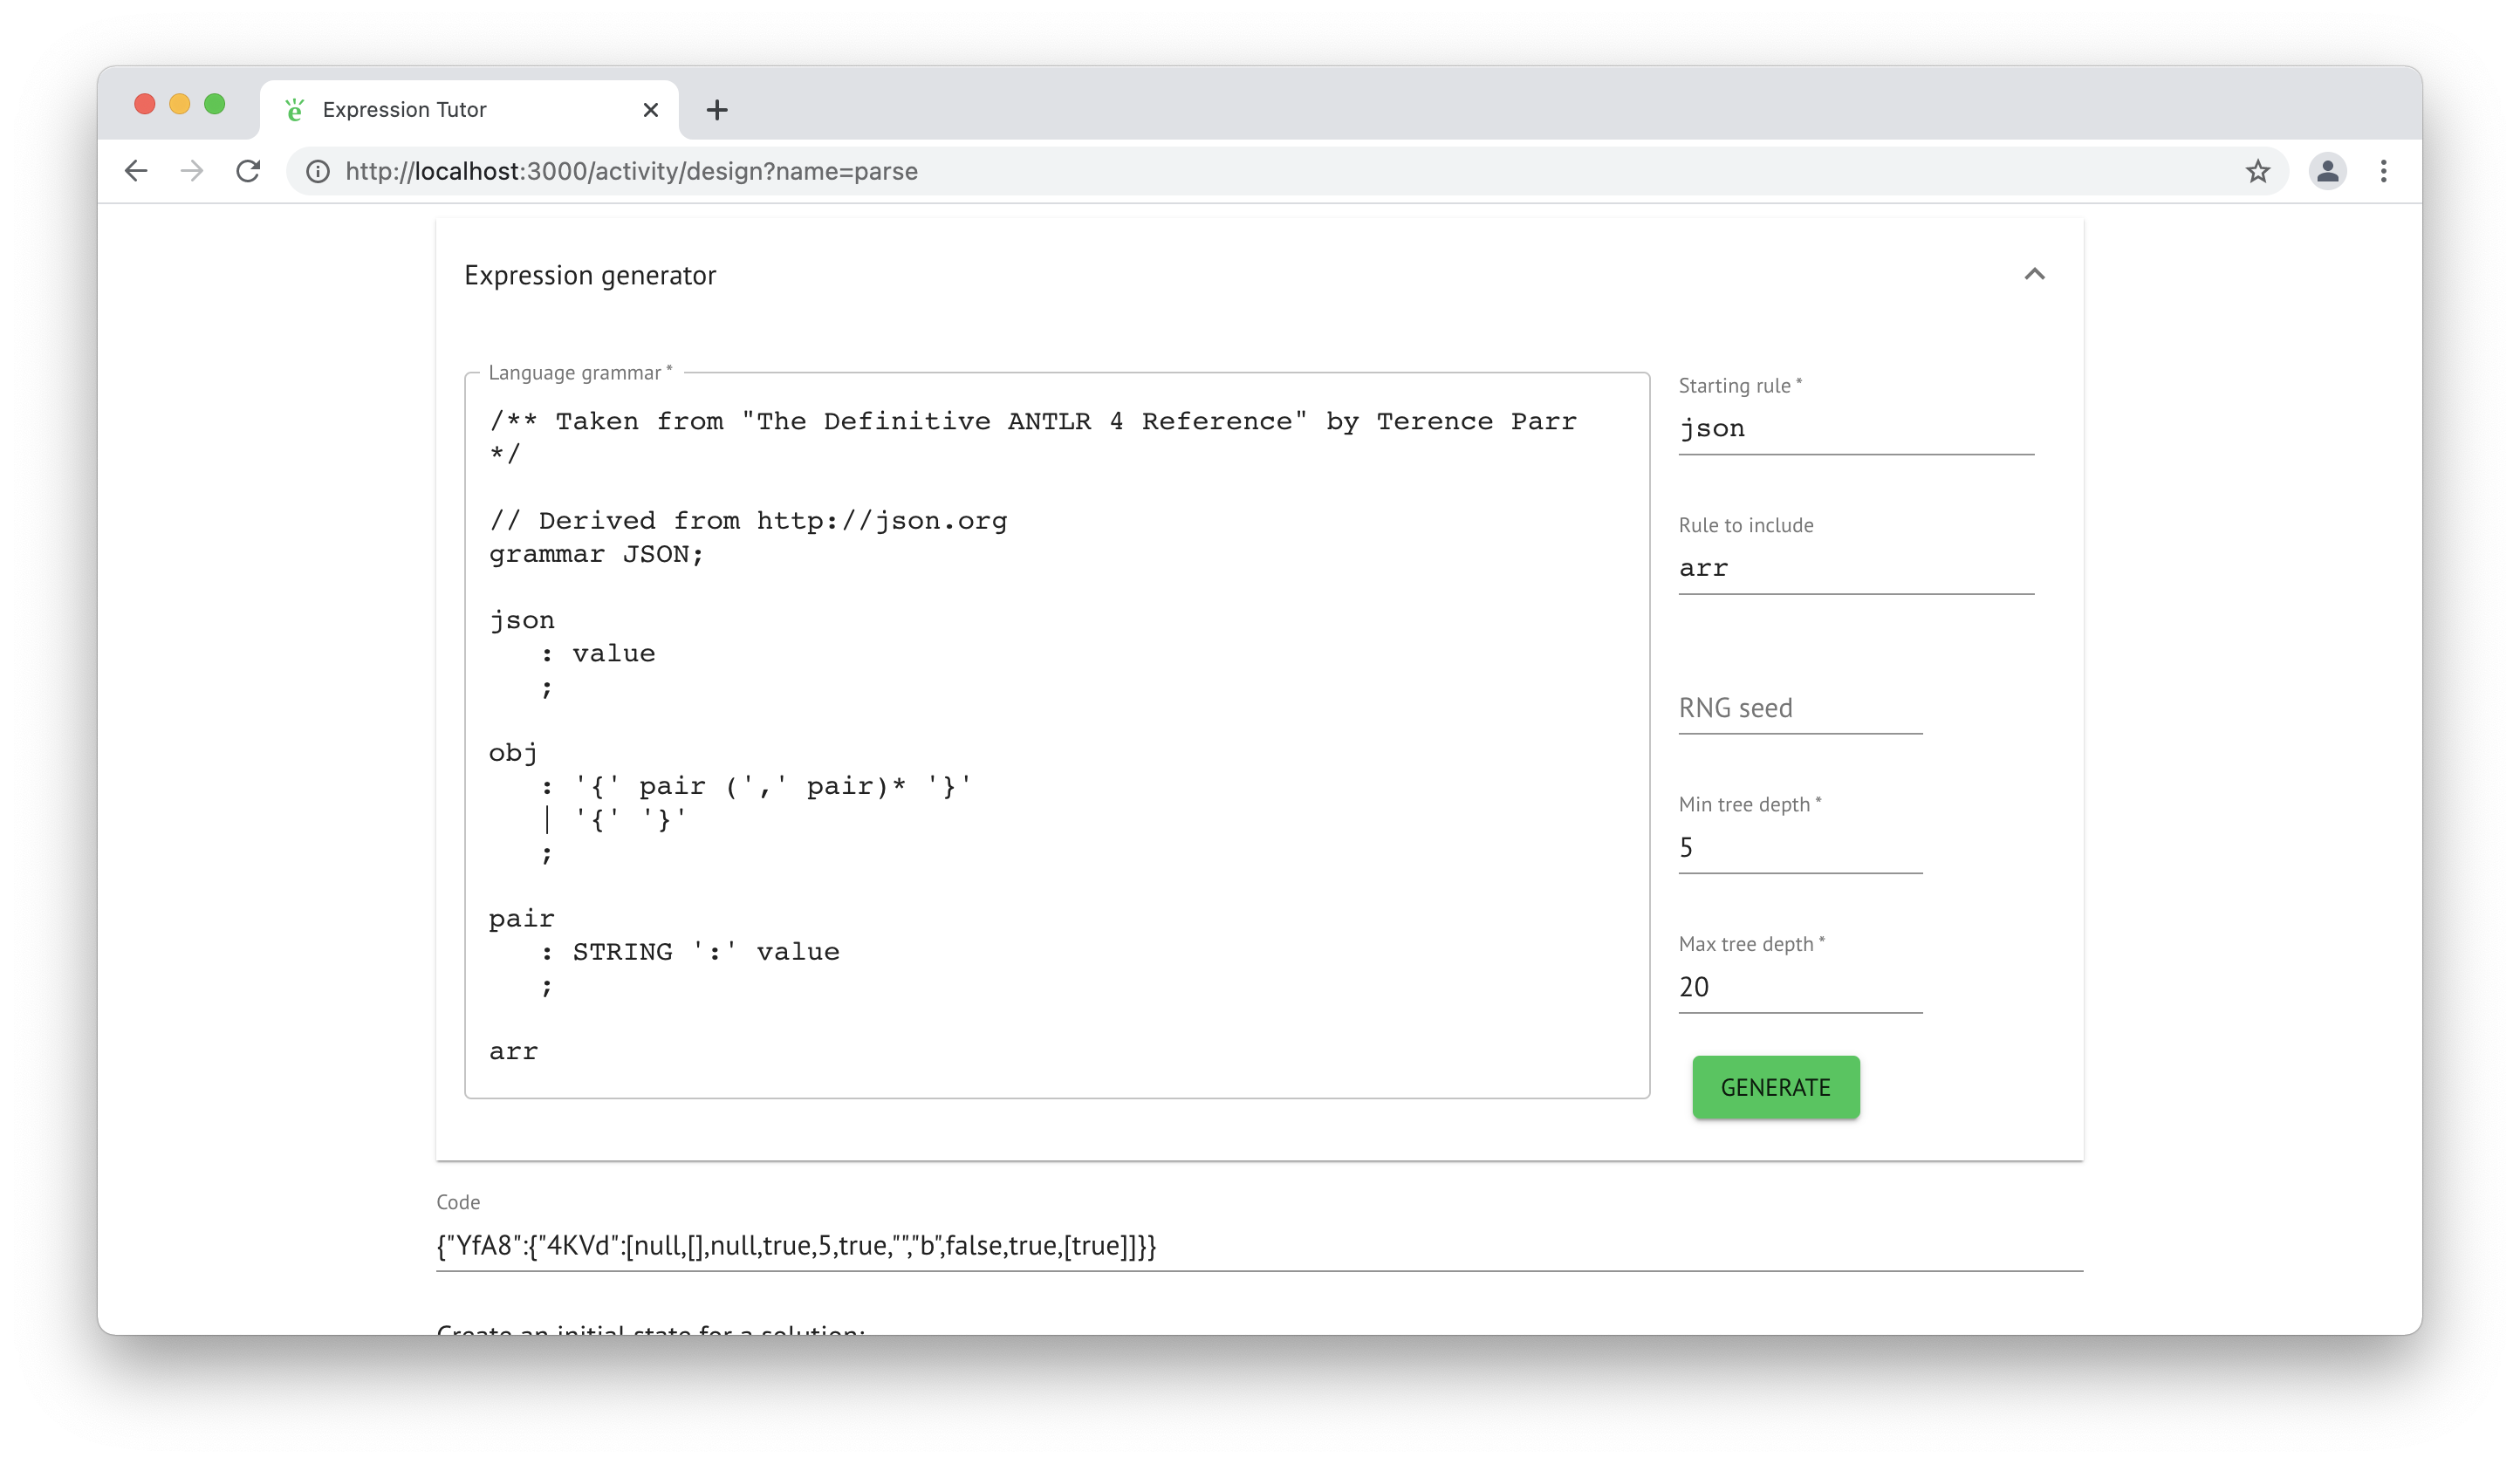
\includegraphics[width=\textwidth]{img/web_tutor_show.png}
\end{frame}

% ------------------------------

% 7.0
\begin{frame}
\frametitle{4. Let's generate an expression}

\begin{enumerate}
\item Get to know the grammar
    \begin{itemize}
    \item ANTLR the wrong way: instead of using its powerful expression parsing
          capabilities, we are only interested in its grammar parsing
    \end{itemize}
\end{enumerate}
\end{frame}

% 7.1
\begin{frame}
\frametitle{4. Let's generate an expression}

\begin{enumerate}
\item Get to know the grammar
    \begin{itemize}
    \item ANTLR the wrong way: instead of using its powerful expression parsing
          capabilities, we are only interested in its grammar parsing
    \end{itemize}
\item Understand the rules\\
    Compute:
    \begin{itemize}
    \item distance between each one of them
    \item distance to shortest terminator
    \item usage relationships
    \end{itemize}
\end{enumerate}
\end{frame}

% 7.2
\begin{frame}
\frametitle{4. Let's generate an expression}

\begin{enumerate}
\item Get to know the grammar
    \begin{itemize}
    \item ANTLR the wrong way: instead of using its powerful expression parsing
          capabilities, we are only interested in its grammar parsing
    \end{itemize}
\item Understand the rules\\
    Compute:
    \begin{itemize}
    \item distance between each one of them
    \item distance to shortest terminator
    \item usage relationships
    \end{itemize}
\item Build a Concrete Syntax Tree
    \begin{itemize}
    \item Pick the next optimal rule alternative given the user constraints:
          routing–like algorithm with a twist
    \item Build each rule following its grammar specification
    \end{itemize}
\end{enumerate}
\end{frame}

% ------------------------------

% 8.0
\begin{frame}[c]
\centering
\Huge Demo
\end{frame}

\end{document}